\documentclass{article}

% if you need to pass options to natbib, use, e.g.:
%     \PassOptionsToPackage{numbers, compress}{natbib}
% before loading neurips_2019

% ready for submission
% \usepackage{neurips_2019}

% to compile a preprint version, e.g., for submission to arXiv, add add the
% [preprint] option:
%     \usepackage[preprint]{neurips_2019}

% to compile a camera-ready version, add the [final] option, e.g.:
     \usepackage[final]{neurips_2019}

% to avoid loading the natbib package, add option nonatbib:
%     \usepackage[nonatbib]{neurips_2019}

\usepackage[utf8]{inputenc} % allow utf-8 input
\usepackage[T1]{fontenc}    % use 8-bit T1 fonts
\usepackage{hyperref}       % hyperlinks
\usepackage{url}            % simple URL typesetting
\usepackage{booktabs}       % professional-quality tables
\usepackage{amsfonts}       % blackboard math symbols
\usepackage{nicefrac}       % compact symbols for 1/2, etc.
\usepackage{microtype}      % microtypography
\usepackage{graphicx}       % display figure
\usepackage{hyperref}       % clickable links

\title{Unsupervised Anomaly Detection in Electrocardiograph Time Series Data Using Variational Recurrent Autoencoders with Attention, and Transformer}

% The \author macro works with any number of authors. There are two commands
% used to separate the names and addresses of multiple authors: \And and \AND.
%
% Using \And between authors leaves it to LaTeX to determine where to break the
% lines. Using \AND forces a line break at that point. So, if LaTeX puts 3 of 4
% authors names on the first line, and the last on the second line, try using

\author{%
  Ke Xu \\
  Electrical and Computing Engineering\\
  Carnegie Mellon University\\
  Pittsburgh, PA 15213 \\
  \texttt{kxu2@andrew.cmu.edu} \\

  \And
  Nicky Nocerino \\
  Electrical and Computing Engineering\\
  Carnegie Mellon University\\
  Pittsburgh, PA 15213 \\
  \texttt{nnocerin@andrew.cmu.edu} \\

  \And
  Yilin Wang \\
  Civil and Environmental Engineering\\
  Carnegie Mellon University\\
  Pittsburgh, PA 15213 \\
  \texttt{yilinw2@andrew.cmu.edu} \\

  \And
  Zhufeng Fan \\
  Civil and Environmental Engineering\\
  Carnegie Mellon University\\
  Pittsburgh, PA 15213 \\
  \texttt{zhufengf@andrew.cmu.edu} \\
  % examples of more authors
  % \And
  % Coauthor \\
  % Affiliation \\
  % Address \\
  % \texttt{email} \\
  % \AND
  % Coauthor \\
  % Affiliation \\
  % Address \\
  % \texttt{email} \\
  % \And
  % Coauthor \\
  % Affiliation \\
  % Address \\
  % \texttt{email} \\
  % \And
  % Coauthor \\
  % Affiliation \\
  % Address \\
  % \texttt{email} \\
}

\begin{document}

\maketitle
%%%%%%%%%%%%%%%%%%%%%%% Abstract %%%%%%%%%%%%%%%%%%%%
\begin{abstract}

Time series data holds a long exists on various field in our daily life. It is hard to extract the pattern of the data by human effort. Since computer intelligence are
expected to perform more sensitive than human beings, deep learning algorithms especially data pattern detection has been applied to detect anomaly pattern from complex system, such as heartbeat signal. However, a significant amount of approaches based on supervised machine learning models that require (big) labelled data-set. In this project, we are expected to detect the pattern of heartbeat with an optimized Auto-Encoder model. Our contributions can be divided as three steps. Firstly, we established two baseline model (MLP and LSTM auto-encoder) on MNIST dataset. The results shows a good sensitivity on distinguish from different data.  Secondly, we add attention machenisms to LSTM decoder to improve the performance. Finally, we use multi-head attentional transformer model instead of LSTM auto-encoder to explore the possibilities of replacement.  We can see a very clear loss threshold between the normal and abnormal data.


\end{abstract}

%%%%%%%%%%%%%%%%%%%%%%% Introduction %%%%%%%%%%%%%%%%%%%%
\section{Introduction}
The time series data are widely used right now. Monitoring heart beat signals with pattern recognition algorithms makes it possible to diagnose heart disease by detecting anomalous behaviours, which contributes to improving the fitness of human bodies. The problem of finding patterns in data that do not conform to expected or normal behaviour is often referred to as Anomaly Detection. Since the mid-1990s, many computer science researchers have been working on how to automatically detect anomalies and many methods have been proposed. In particular, recently researchers have successfully built some robust deep learning models with large dataset to detect anomalies. 

However, a significant amount of these approaches are based on supervised machine learning models that require (big) labelled datasets to be trained. Furthermore, some of the proposed methods do not consider the sequential nature of the data by assuming it is independent in time. To address the above issues, Joao Pereira and Margarida Silveira proposed a method called Variational Recurrent Autoencoders with Attention \cite{AuthorJM}, which uses time series data to train an unsupervised model. 

Our project is based on Joao Pereira and Margarida Silveira's work. First, we will implement a pure LSTM network refering to their model and replicate experimental results. This will be our first model, or in other word, baseline model. Then we will try to improve the performance of the model by individually adding attention layers and replacing with transformer model. Finally, we will compare the performance of the three models on the accuracy as a "classifier" of abnormal patterns from a mixed test dataset. 

%%%%%%%%%%%%%%%%%%%%%%% Literature Review %%%%%%%%%%%%%%%%%%%%
\section{Literature Review}
In recent years, various machine learning methods have been applied widely to automate the process monitoring and fault diagnosis. Artificial neural networks are popular due to a simplicity in logic and a powerful ability to deal with nonlinear problems such as abnormally detection. Typical supervised learning method with various build-in structures, for example, multi-layer perceptron (MLP) \cite{AuthorSI}, learning vector quantization networks (LVQ), were used to detect simple patterns such as shift, trend, cycle etc. With a further development of the network structure, hybrid model with a combination of models come into appear.

\subsection{Abnormally detection}
Abnormally detection has been widely used on system control and management. Potes and Cristhian development of an algorithm to classify normal/abnormal heart sounds from the observation dataset on human bodies. A total of 124 time-frequency features were extracted from the phonocardiogram (PCG) which is used as an input of a convolutional neural network (CNN) based on an ensemble of classifiers combining the outputs of AdaBoost. \cite{AuthorPotes} Du and Min (2017), proposed a Long Short-Term
Memory (LSTM), to model a system log as a natural language sequence. With and automatic learning from log patterns, it allowed the algorithm to detect anomalies when log patterns deviate from the model trained from log data under normal execution. \cite{AuthorDu}

\subsection{Auto-encoder (AE) and Auto-decoder (AD) network}
With addressing a large scale of data and high-dimensional level of learning, autoencoder (AE) makes its way into health monitoring \cite{AuthorRZ}, fault diagnosis AE models could learn representative features from raw data by reconstructing input data from an artificial corruption. For years, AE models have been widely used on diverse fields to deal with the practical problem. Chen, Min, et al (2017), proposes a convolutional autoencoder deep learning framework to support unsupervised image
features learning for lung module with a small amount of labeled data for efficient feature learning. Kamper and Herman (2015), proposed an unsupervised neural network feature extractor without resources in zero-resource settings. They achieved a two-third of relative improvement with the feature extractor in a word discrimination task. \cite{AuthorKa} Fan and Cheng (2018) investigates the potential of autoencoders in detecting anomalies in building energy data. Specific methods have been
designed to evaluate the autoencoder performance, the results can be used as foundation for building professionals to develop advanced tools for anomaly detection. 



%%%%%%%%%%%%%%%%%%%%%%% Contribution %%%%%%%%%%%%%%%%%%%%
\section{Contribution}
In this project, our contributions are about to optimize the time-series auto-encoder with transformer learning and attention layer to speed-up the training process and optimize the accuracy. In this section, we will firstly discuss how the LSTM auto-encoder works, then we will talk about what the obstacle is and, finally, we will present how transformer and attention works on our project model.

\subsection{Problem Restatement}
Overall, recurrent models factor computation along the symbol positions of the input and output
sequences. The performances of the network become critical when the size of sequence batches are longer as functions of previous hidden state precludes parallelization within training examples. This issues cannot be properly solved only with changing the parameters. 

In the process of detecting abnormally signals from time-series data by auto-encoder. The result of the encoders is greatly affected by the context information. In our project, since heart beating signal is repeatedly continuous in a given period of time, the signal of heart beating has a clear pattern to distinguish abnormal beating from normal beating signal. However, the differences between heart beating data from language model is the beating patterns are not determined by historical beating but have the connections instead. With a conventional auto-encoder, which majorly weights the relationships between sequence data, it would take much time to extract features and train the data

\subsection{Attention-based Auto-encoder}
Out first optimization model a recursive neural network auto-encoder with one sequence-to-sequence attention model. Attention Mechanism allows the decoder to dynamically focus on the information-rich phrases in the source sequence by taking a peek at the encoder states that are relevant to the current decoding step. It allows the algorithms to pay a distributed attentions on between different parts of the source sequence at different decoding steps. In our model, we are implementing "dot-product" attention mechanism to achieve this. 

The first step in calculating self-attention is to create three vectors from each of the encoder’s input vectors (in this case, the embedding of each data points). So for each word, we need a Query vector, a Key vector, and a Value vector. These vectors are created by multiplying the embedding by three matrices that we trained during the training process.

The next step to calculate attention is to get the score. Score is a numerical measurement on how much the algorithms should focus to data other than the input sentence at a certain position. 

The calculating function is: score = $q_{i}$\cdot$k_{i}$ where $i$ represents the i-th data points

\begin{figure}[!t]
    \centering
    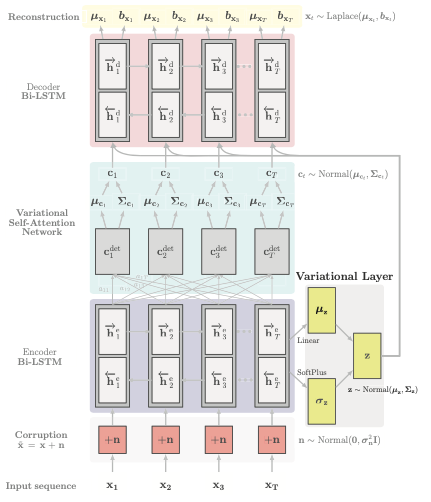
\includegraphics[width=0.7\textwidth]{images/BiLSTM.png}
    \caption{Variational Bi-LSTM Autoencoder with Variational Self-Attention.}
\end{figure}


\subsection{Transformer Model}

Most competitive neural sequence transduction models have an encoder-decoder structure. In general, the architectures of encoder network and decoder network are similar in a traditional auto-encoder model. Thus, it provides a possibility to transformer the encoder as decoder to generate the entire auto-encoder model. However, traditional encoder continuously maps the input sequence and then generate the sequence by decoder, which will take to much computational resources.

Transformer model, on the other hand, follows the overall architecture using stacked self-attention and point-wise, fully connected layers for both the encoder and decoder. The decoder is transformed by encoder. The structure of Transformer model is showed in Figure below. This figure is cited from paper named "Attention is All You Need" 

\url{https://arxiv.org/abs/1706.03762}









\begin{figure}
    \centering
    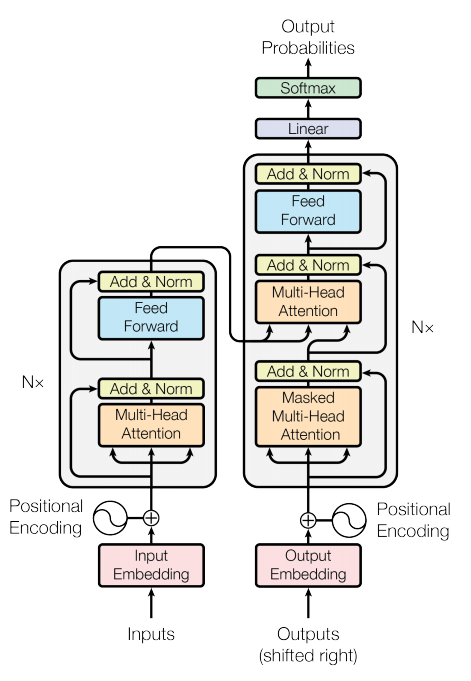
\includegraphics[width=0.7\textwidth]{images/The Transformer Model Architecture.png}
    \caption{The Transformer-model Architecture}
\end{figure}


Multi-head attention mechanism is a improved attention mechanism. It can be described as mapping a query and a set of key-value pairs to an output, where the query, keys, values, and output are all vectors. A expected output of the transformer model is a weighted sum of the weights, which is generated from multi-head attention mechanism. Figure-2 describes the basic steps of multi-head attention in work-flow chart, which is cited from the blog(\url{http://jalammar.github.io/illustrated-transformer/}).

\begin{figure}
    \centering
    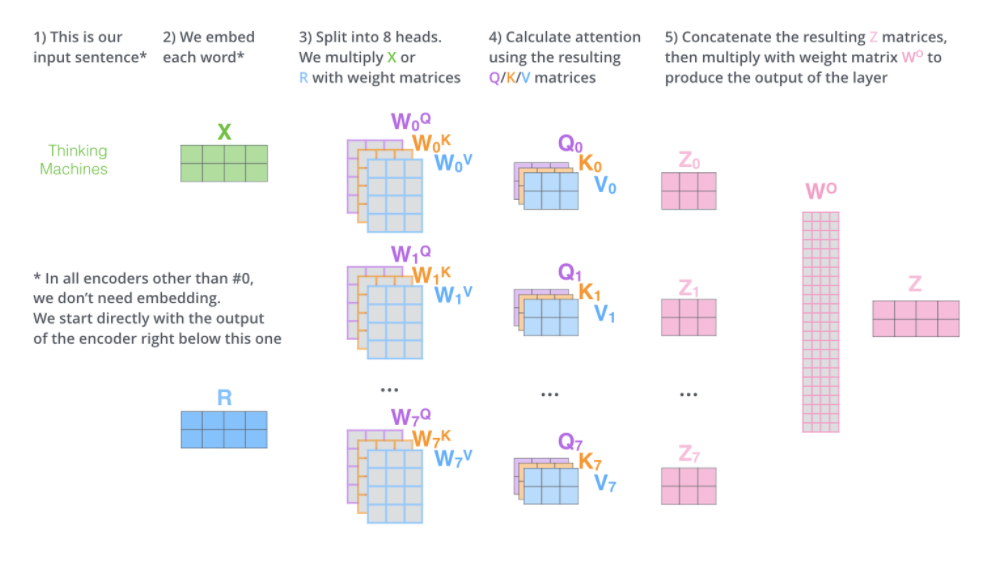
\includegraphics[width=0.9\textwidth]{images/Calculations on Attention Vector on Multi-head Attention Model.png}
    \caption{Calculations on Attention Vector on Multi-head Attention Model}
\end{figure}


Compared with the conventional attention-based layer, it has two major advantages.

\begin{itemize}
    \item Multi-head attention algorithms can expand the focus on different positions. As each data points generate their own attention vector called $z_{i}$, where $i$ represents the index of the current data point. Every data point, which is the heart beat value at exact time spot, holds its unique attention vectors on the data at other time spot instead of share one attention vector with one head. As time series heart beating data has less context effect between the adjacent data point than language data, multi-head attention generate individual attention relationship without cutting out the connection between the time-series data. 
    \item Multi-head attention provides multiple subspace to store the "attention vectors". As showed in Figure 3 and Figure 4, multiple sets of Query/Key/Value weight matrices represent attention with individual random initialization and training.
\end{itemize}

\begin{figure}
    \centering
    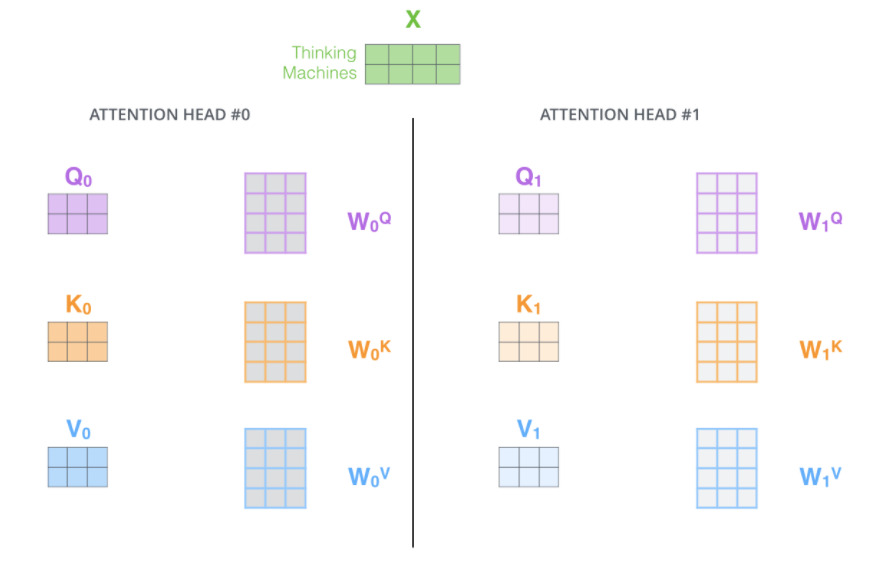
\includegraphics[width=0.9\textwidth]{images/Multiple Attention Subspace.png}
    \caption{Multiple Attention Subspace}
\end{figure}

\subsection{Model Implementation}

All of the models are trained using normal data, and in order to get a better testing result, testing normal data and abnormal data should have the same size. In the ECG data case, 2919 heartbeats among 4500 training data are used for training, and 352 among 500 heartbeats are selected for testing, since there are only 176 normal test data and we pick another 176 abnormal data as counterpart.

Model details:

\begin{itemize}
    \item LSTM AutoEncoder (Fig5)\\
    Encoder: \\
    LSTM(inputsize=1, hiddensize=128, layers=1)\\
    LSTM(inputsize=128, hiddensize=64, layers=1) \\
             
    Decoder: \\
    LSTM(inputsize=64, hiddensize=64, layers=1)\\
    LSTM(inputsize=64, hiddensize=128, layers=1)\\
    Linear(128, 1) \\
    
    Optimizer: Adam(learning rate = 1e-3)\\
    Loss: L1 Loss (mean absolute error)
    
    
    \item LSTM AutoEncoder with Attention (LSTM layers are bi-directional) (Fig6) \\
    Encoder: \\
    LSTM(inputsize=1, hiddensize=128, layers=2)\\
    key network: Linear(256, 128) \\
    value network: Linear(256, 128) \\
             
    Decoder: \\
    LSTM(inputsize=128, hiddensize=128)\\
    LSTM(inputsize=128, hiddensize=128)\\
    Attention(key size = 128; value size = 128)\\
    output layer: Linear(256, 1) \\
    
    Optimizer: Adam(learning rate = 1e-3)\\
    Loss: L1 Loss (mean absolute error) \\

    \item Transformer \\
    Embedding layer: Linear(1, 64) \\
    Transformer layer: Transformer(input features=64) \\
    Output layer: Linear(64, 1) \\
    
    Optimizer: Adam(learning rate = 1e-3)\\
    Loss: L1 Loss (mean absolute error) \\
    
\end{itemize}

\begin{figure}
    \centering
    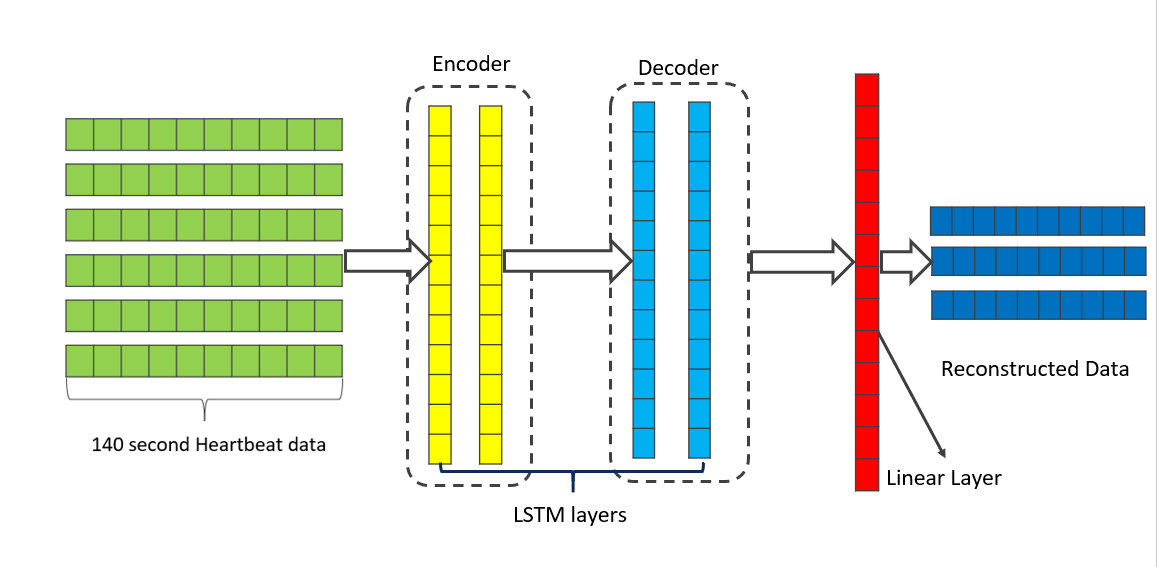
\includegraphics[width=0.9\textwidth]{images/lstmautoencoder.png}
    \caption{LSTM autoencoder architecture}
\end{figure}

\begin{figure}
    \centering
    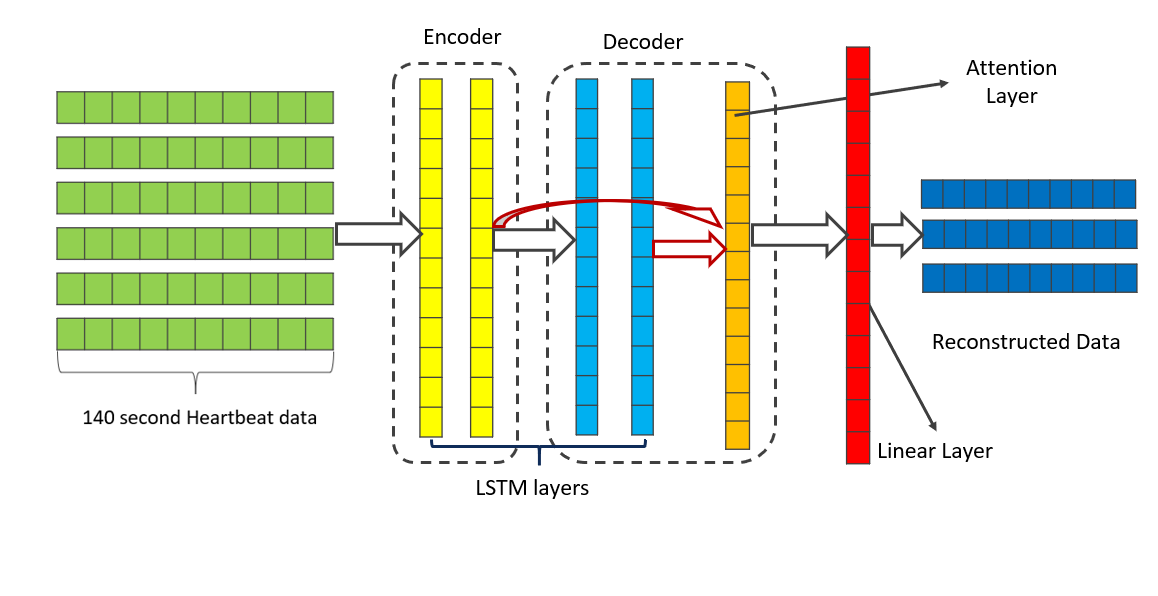
\includegraphics[width=0.9\textwidth]{images/lstmautoencoderattention.png}
    \caption{LSTM autoencoder with attention architecture}
\end{figure}




%%%%%%%%%%%%%%%%%%%%%%% Experiment %%%%%%%%%%%%%%%%%%%%
\section{Experiment Evaluation}

\subsection{Experiments}
Here is the link of our project:\href{https://github.com/Dylan-Wyl10/11-785-20F-project}{11785 project} 


The baseline model shows the autoencoder can successfully detect abnormal time series and our evaluation metrics could provide a useful and effective appealing. In order to improve our detection model performance and exploit its ability of capturing feature information from input, according to the ideas described above, we built an attention-based LSTM autoencoder model and a transformer model. 

During implementing, we met a lot of tricky problems and bugs and we used some tricks to overcome these roadblocks. The most representatives are the following points: 1) The input time series has 140 time length and the encoder captures its information and project it into a 128-dim space. But how to decode the projected features in practice? We solve this by repeating the 128 encoded vector for 140 times and transpose it, feed into the Decoder which has symmetrical structure with the Encoder and transpose back. Such operations ensures that the decoder can generate similar time-series data as the encoder input. 2) The LSTM autoencoder has a smooth learning curve before adding attention, but the attention-based LSTM autoencoder can't always converge  due to model training randomness. We solve this by training more times, and under most circumstances it is able to converge at a specific loss.

Assumptions we made: \\
For the time-series anomaly detection problem, we use normal heartbeats to train the model, then the test loss of abnormal heartbeats will be much higher than normal heartbeats. We assume there is an expected threshold to classify normal and abnormal time-series according to test loss, and such "classification" can be clearer when a more advanced model is being used. We also assume that the length of time series is long enough so the attention-based model is able to converge.\\

We developed our models from scratch using pytorch. We also refer to some online sources for some of the drawing code.

\subsection{Dataset}
\subsubsection{MNIST}
The "mnist" dataset is a public image database of handwritten digits that is commonly used for training various image processing systems. Our goal is to test the performances of our baseline anomaly detection model by feeding the images from mnist dataset.
\url{https://en.wikipedia.org/wiki/MNIST_database}

This dataset is very small. It won't take a long time to trian our model and we can easily add noise to the test images to create abnormal data. That's why we choose to use mnist for our baseline models. Firstly, a dataset with noises is supposed to be generated. We selected 1000 samples from the test data and added random noise. Gaussian noise is applied in this case. Then we conbine the 1000 abnormal data with the remaining 9000 clean data to form an abnormal test dataset. We will use the
train data of mnist dataset to train our model and abnormal test data to test whether our autoencoders can successfully detect the abnormality.

\subsubsection{ECG5000}
The dataset we choose is a Electrocardiograph (ECG) data, which is a 20-hour-long time-series data originally from Physionet[ref]. We download this data from a public data source named Time Series Classification[ref]. The author has pre-processed the data by extracting each heartbeat then interpolating to make them equal length. 5,000 heartbeats are randomly selected and has been split into train data (4500 heartbeats) and test data (500 heartbeats), each of which has a time series length 140 and a column indicating normal/abnormal classification condition, shown as fig7. 2919 heartbeats are normal data which could be fed into autoencoder and other 4 classes are abnormal heartbeats behaviours. Fig8 represents the typical pattern of each label class, showing that the normal data has different distribution pattern than abnormal data.  
\begin{figure}[!t]
    \centering
    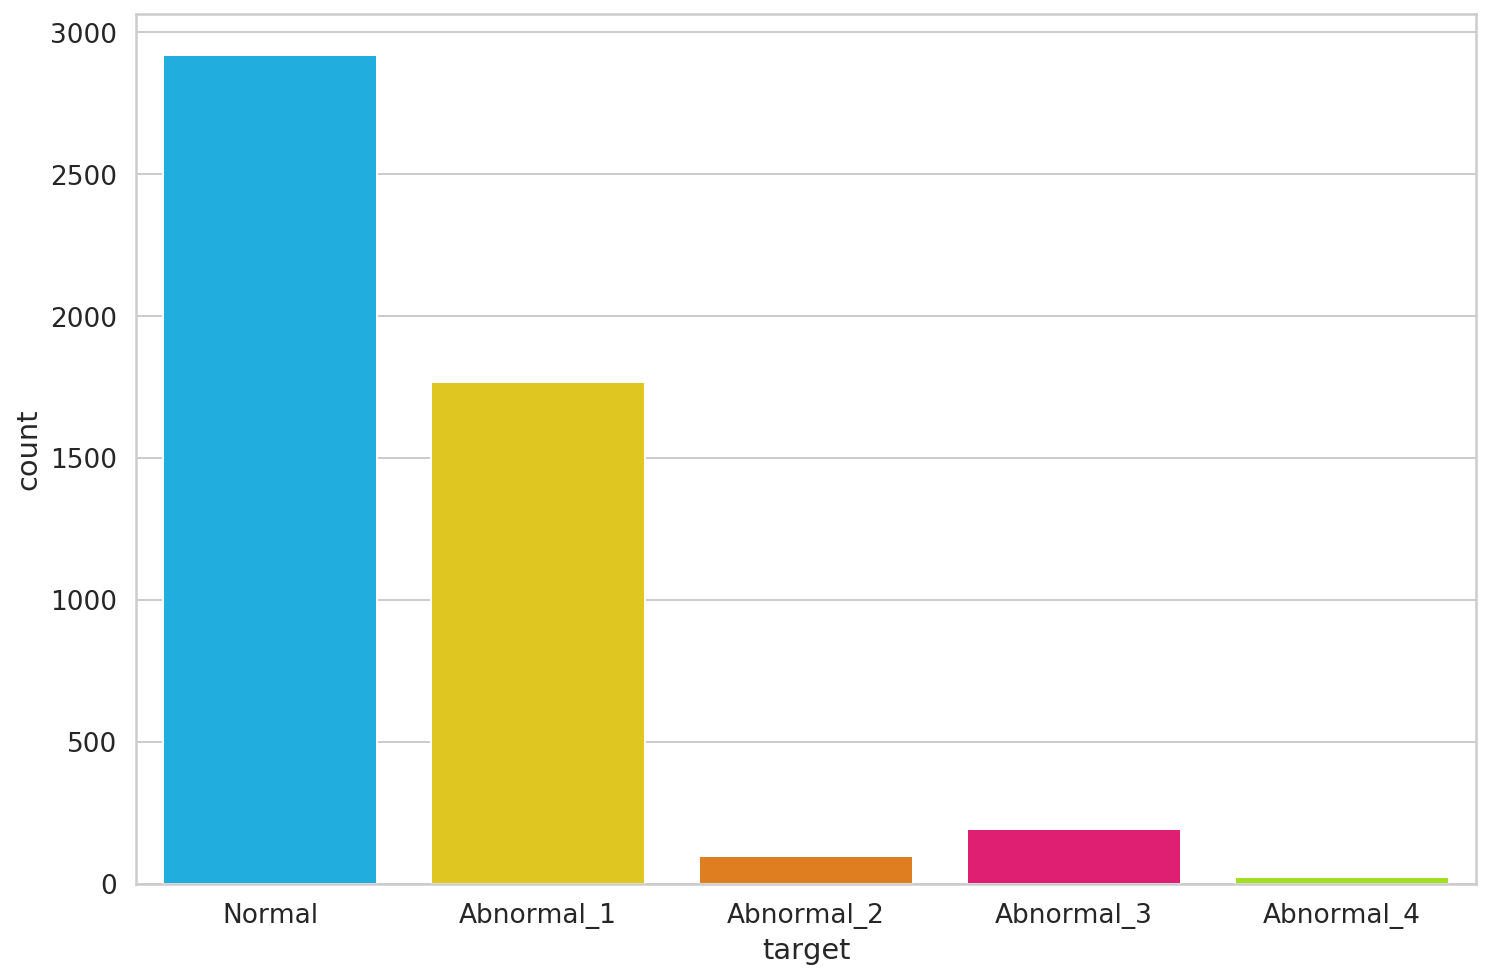
\includegraphics[width=0.7\textwidth]{images/download.png}
    \caption{train dataset normal/abnormal classification.}
\end{figure}
\begin{figure}[!t]
    \centering
    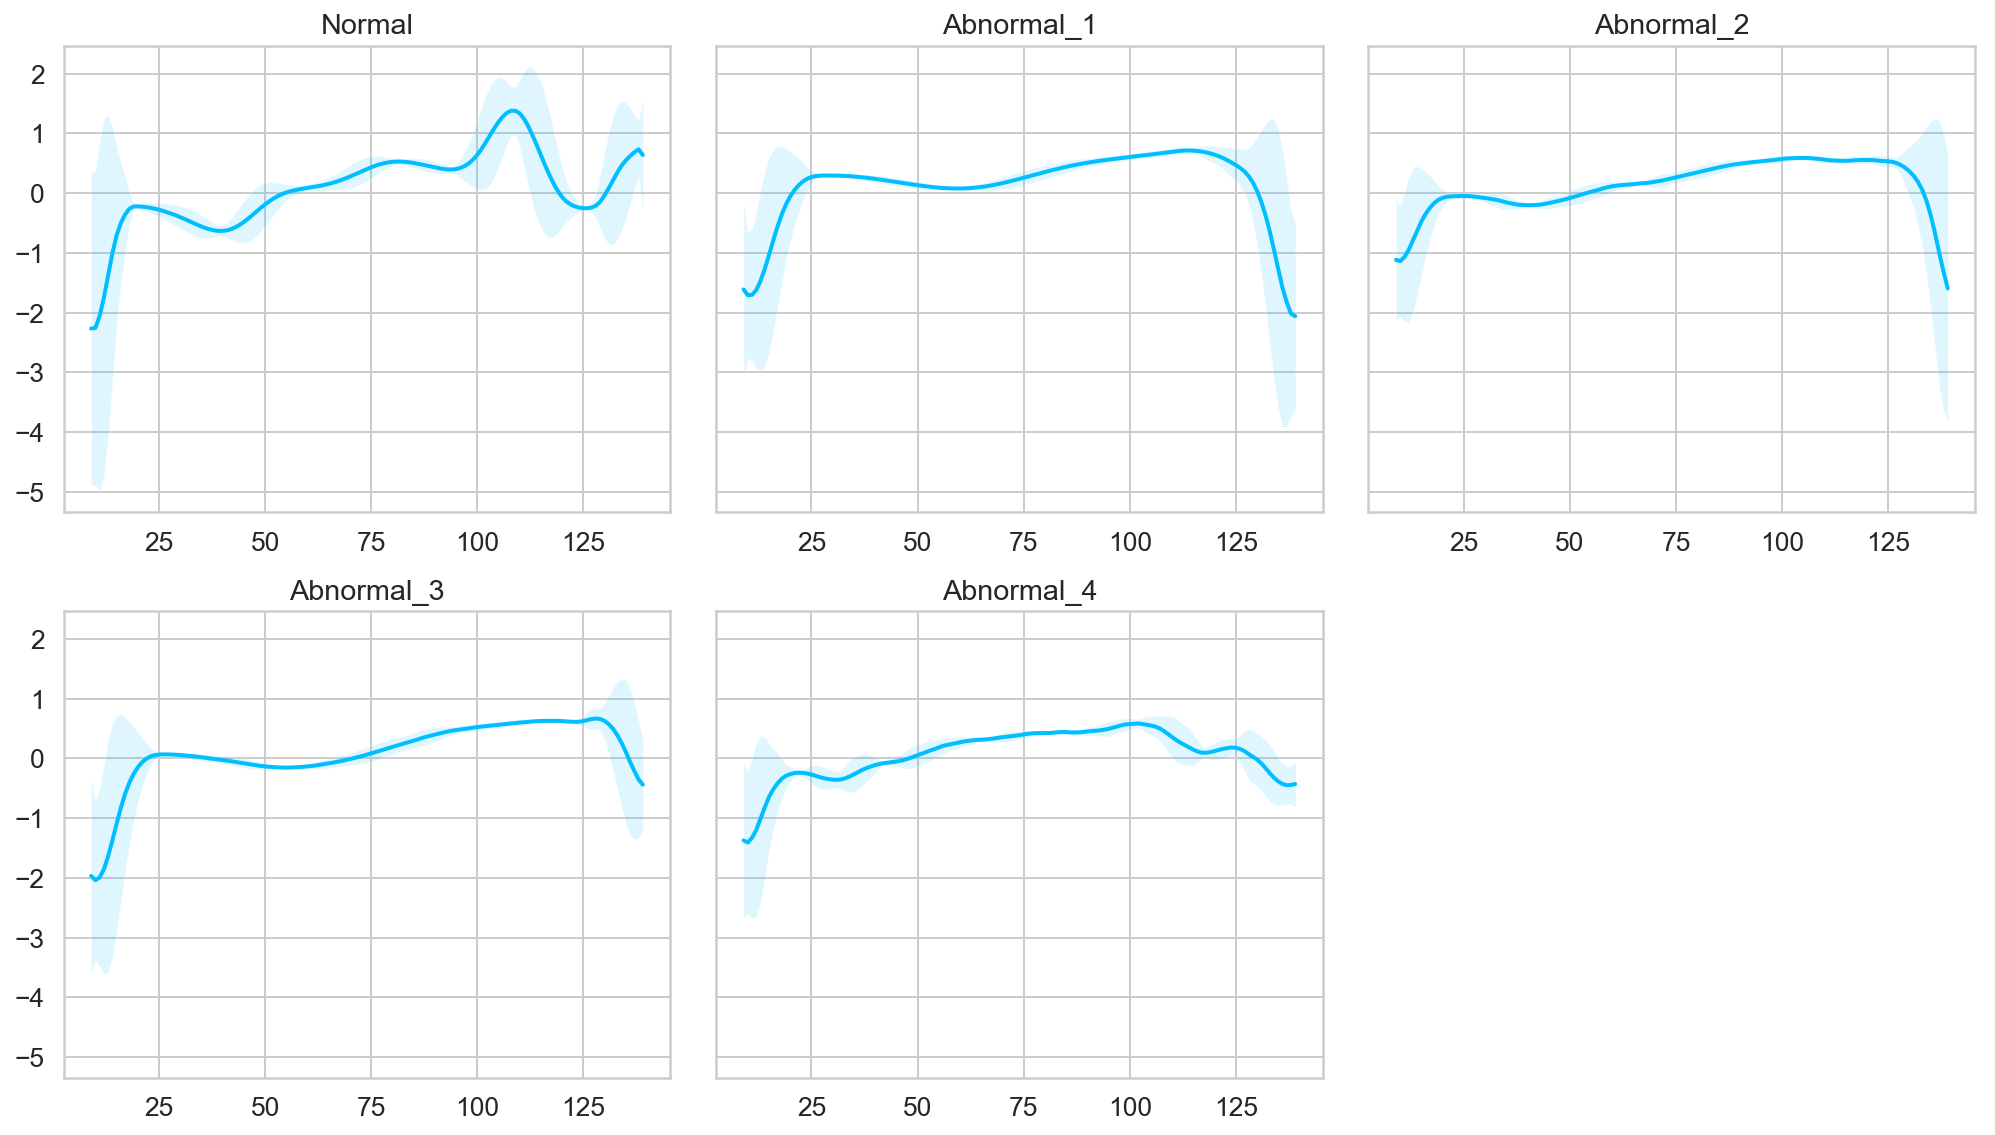
\includegraphics[width=1\textwidth]{images/download (1).png}
    \caption{train dataset normal/abnormal pattern.}
\end{figure}


\subsection{Evaluation Matrix}
Confusion matrix, also known as an error matrix, is a specific table layout that allows visualization of the performance of an algorithm. A classic confusion matrix is a $2\times 2$ table with four attributes, each of which are listed as TP (True Positive), TN (True Negative), FP(False Positive) and FN(False Negative). Table 2 shows the detailed definition of the matrix. (see the url: \url{https://en.wikipedia.org/wiki/Confusion_matrix})

Considering the expected results of anomaly detection is binary, choosing confusion matrix as the evaluation Matrix would be a good way to visualize the performance of the detection model neat and tidy. 

\begin{table}
  \caption{Confusion Matrix of supervised learning}
  \label{obd data}
  \centering
  \begin{tabular}{cccc}
    \toprule
    \multicolumn{3}{c}{True Condition}                   \\
    \cmidrule(r){1-3}
    & Condition positive & Condition negative      \\
    \midrule
    Predicted positive & $TP$ & $FP$     \\
    Predicted negative & $FN$ & $TN$       \\
    \bottomrule
  \end{tabular}
\end{table}

\subsection{Description of baseline}
We first built a MLP autoencoder to test the performance of the autoencoder and whether our evalution metrics works well. Next we built a LSTM autoEncoder to capture the high-level information of input data instead of MLP, because our final model will be based on RNN, which can help us to caputer the features of the time-series data. We want to test whether RNN architectures works well in the autoencoder. We first use our own noise-added mnist dataset on both models and see whether our assumption is valid, then extend to the real-world ECG5000 dataset. 


\subsubsection{MLP-Baseline}
Under the context of baseline Dataset (MNIST), the encoder and decoder architectures of MLP, built using Pytorch: 
\begin{itemize}
\item Encoder: \\
Linear (28*28, 128) + ReLU \\
Linear (128, 64) + ReLU \\
Linear (64, 12) + ReLU \\
Linear (12, 3) \\
\item Decoder: \\
Linear (3, 12) + ReLU \\
Linear (12, 64) + ReLU \\
Linear (64, 128) + ReLU \\
Linear (128, 28*28) + ReLU \\
Loss: MSE loss \\
\end{itemize}
Optimizer: SGD, learning rate=1e-2, weight decay=1e-5, momentum=0.9, train 3 epochs.\\
We choose this model because it could map image data into a relatively small latent space using few linear layers and hidden neurons, which could made training fast and require not too many parameters. 
However, the MLP model is not able to generate latent space for time-series data without context augmentation. So we also built a Bi-LSTM AutoEncoder, which include a LSTM layer and a Linear layer in both encoder and decoder.  

\subsubsection{LSTM-Baseline on MINST}
Under the context of baseline Dataset (MNIST), the encoder and decoder architectures of Bi-LSTM, built using Pytorch: 
\begin{itemize}
\item Encoder: \\
LSTM (28, 256, 3)  \\
Linear (512, 12) \\
\item Decoder: \\
LSTM (12, 256, 3)  \\
Linear (512, 28) \\
Loss: MSE loss \\
\end{itemize}
Optimizer: SGD, learning rate=1e-2, weight decay=1e-5, momentum=0.9, train 3 epochs.\\
Compared to the MLP-Baseline model, Bi-LSTM gives us a larger gap between the loss of clean and abnormal test data, which means it can discriminate the clean and abnormal data better.

\subsubsection{LSTM AutoEncoder on ECG5000}
Described at Model Implementation section in Contribution

\subsubsection{Assumptions}
Several assumptions have been made to narrow down the scope of the baseline experiment. The main objectives is to test the model, thus the assumptions are not considering the closeness between model and real world.
The assumptions are as below:
\begin{itemize}
    \item In our MINST test, images with Gaussian noise can be considered as abnormal data.
    \item In this experiment, we will use a fixed range of threshold as a classifier to distinguish the normal data and anomaly data. In other word, the threshold is expected to perfectly classify the clean and abnormal data. 
\end{itemize}

\subsubsection{Caveats}
The concept of abnormality is very hard to define and have a lot of different forms. Detecting otherabnormalities may not have such a good performance compared to detecting tha abnormality ofadding Gaussian noise



\section{Result}

\subsection{LSTM AutoEncoder}
Using the LSTM autoencoder on ECG5000 data and based on our assumption, we are able to recognize abnormal heartbeats based on decoder test loss distribution. Fig9 and Fig10 represent loss distribution on normal and abnormal data separately. We then pick a threshold 25 for normal/abnormal data prediction classification (i.e. normal for less than 25; abnormal for more than 25). Comparing to labels, we can draw a Confusion matrix, shown as Fig11. From the reconstruction curve(fig12), we can observe that the antoencoder successfully captures features from normal input data, and can distinguish abnormal ones when it comes into the autoencoder.

\begin{figure}[!t]
    \centering
    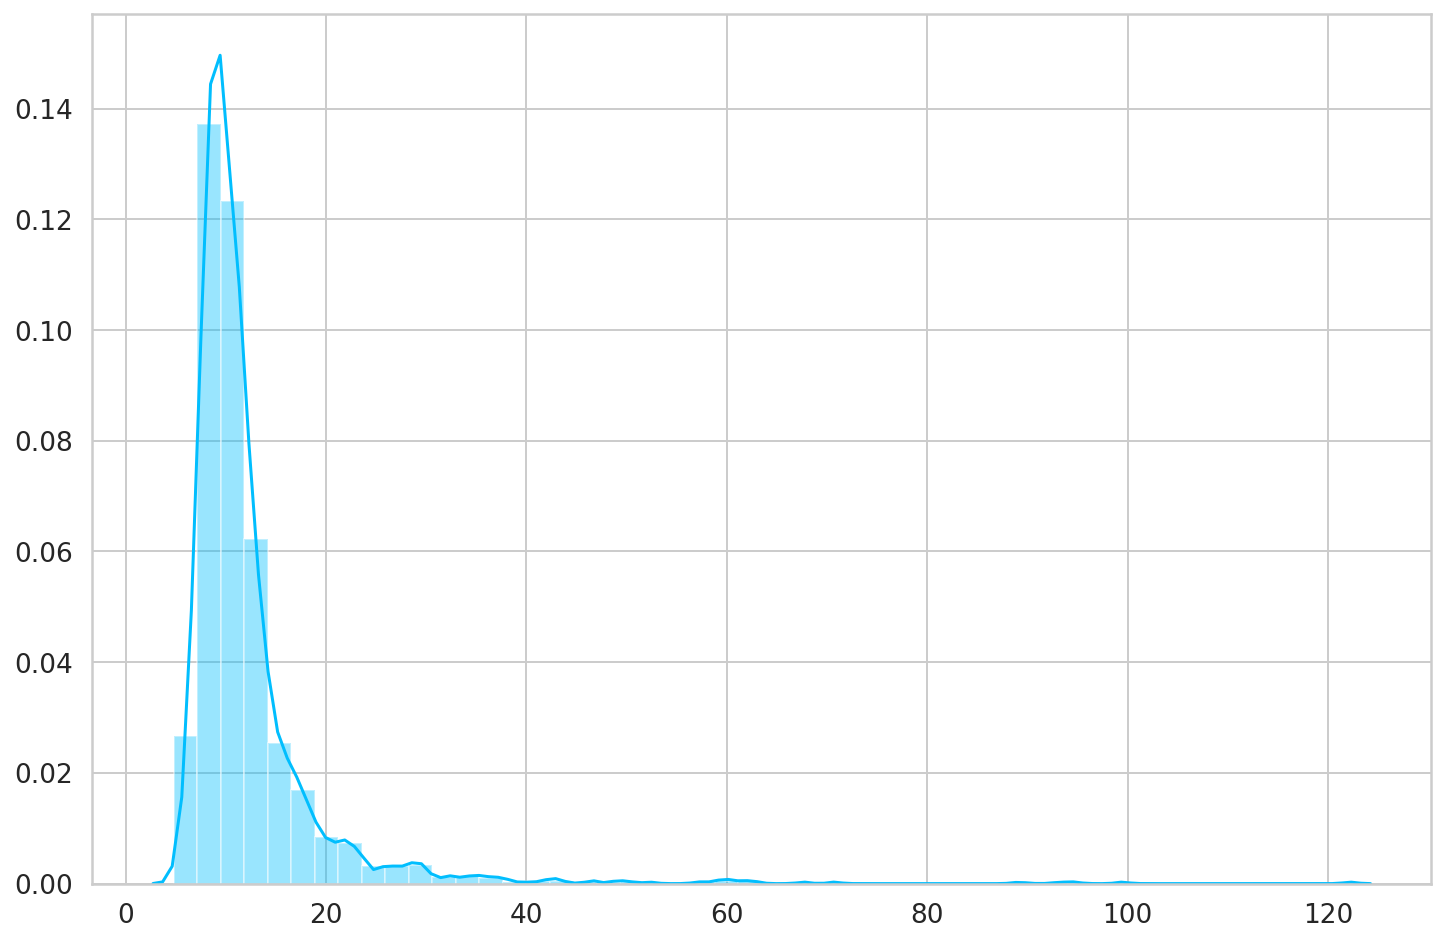
\includegraphics[width=0.7\textwidth]{images/baseline_normal.png}
    \caption{LSTM Autoencoder: normal heartbeats loss distribution.}
\end{figure}

\begin{figure}[!t]
    \centering
    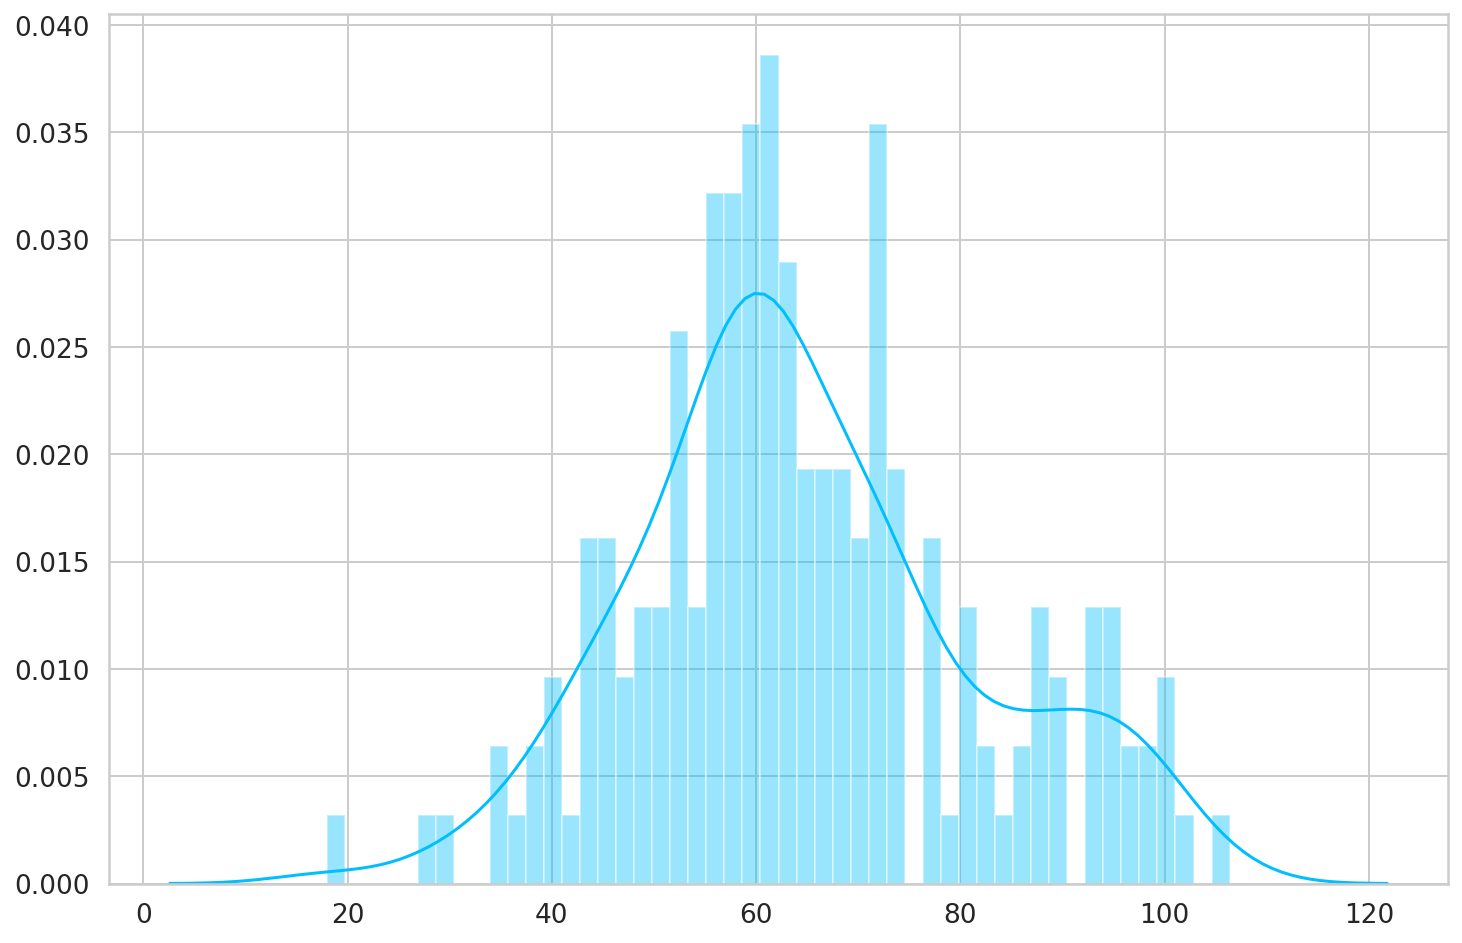
\includegraphics[width=0.7\textwidth]{images/baseline_abnormal.png}
    \caption{LSTM Autoencoder: abnormal heartbeats loss distribution.}
\end{figure}

\begin{figure}[!t]
    \centering
    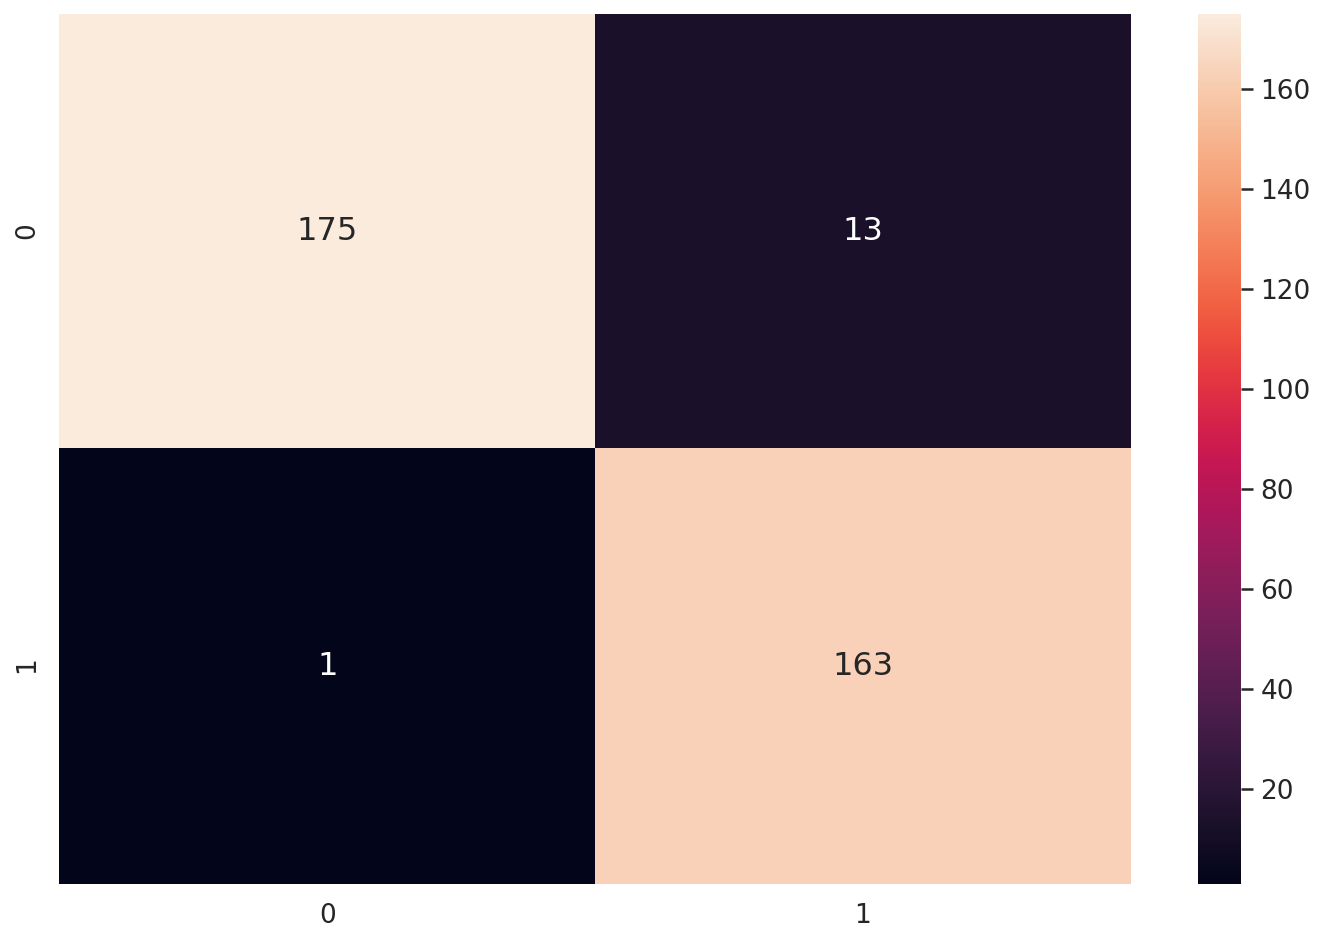
\includegraphics[width=0.7\textwidth]{images/baseline_Cofmat.png}
    \caption{LSTM Autoencoder: Confusion Matrix.}
\end{figure}

\begin{figure}[!t]
    \centering
    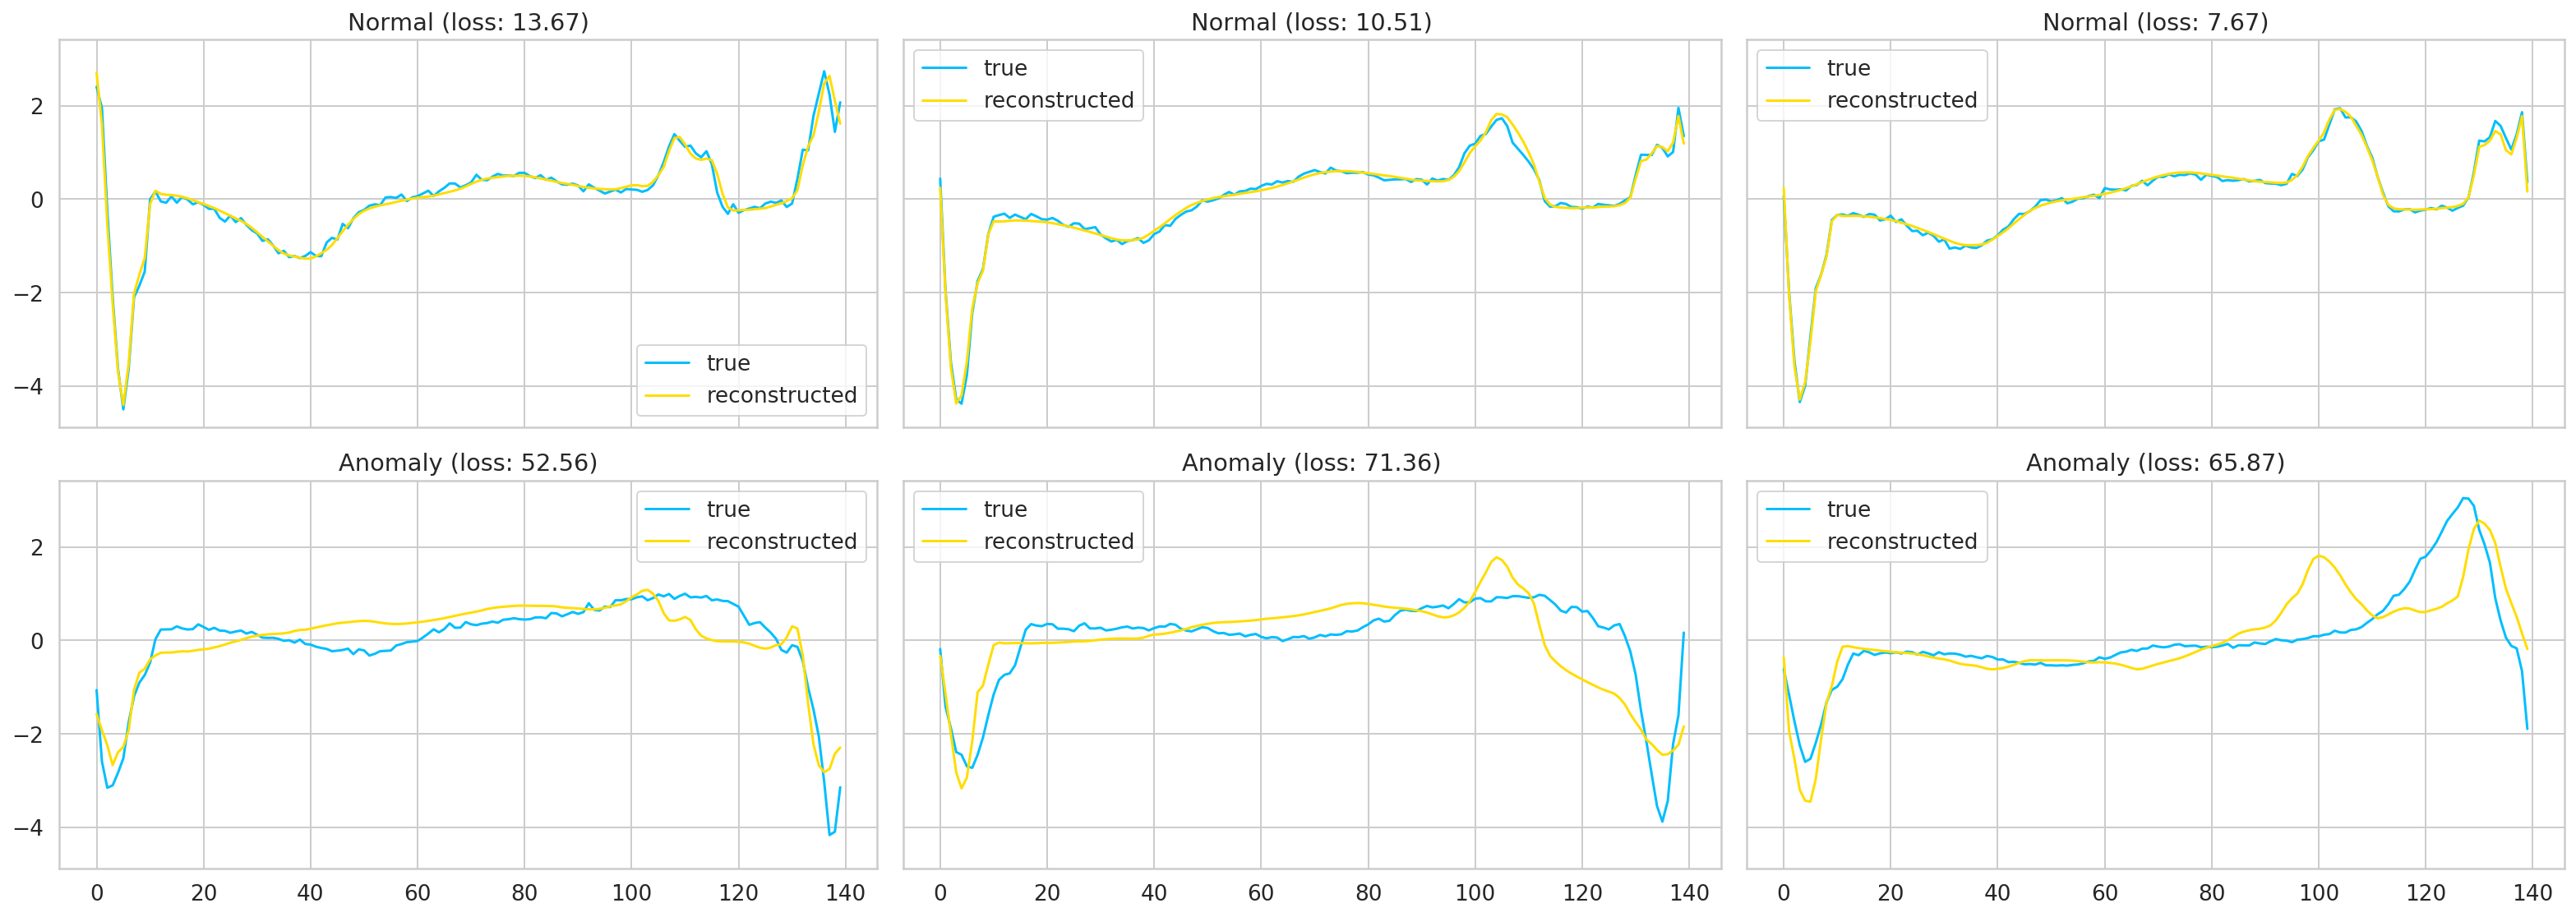
\includegraphics[width=1.0\textwidth]{images/baseline_reconstruct_curve.png}
    \caption{LSTM Autoencoder: reconstruction.}
\end{figure}

\subsection{LSTM Autoencoder with Attention}
After applying for attention mechanism, the abnormal detection ability has improved. From Fig13 and Fig14 we can find a wider and clearer classification threshold range than the model without attention. Confusion matrix (Fig15) verified this. With attention, only 4 heartbeats are misidentified. The Attention mechanism significantly increases the ability of feature identification in normal data and the capability to recognize anomaly time series.

\begin{figure}[!t]
    \centering
    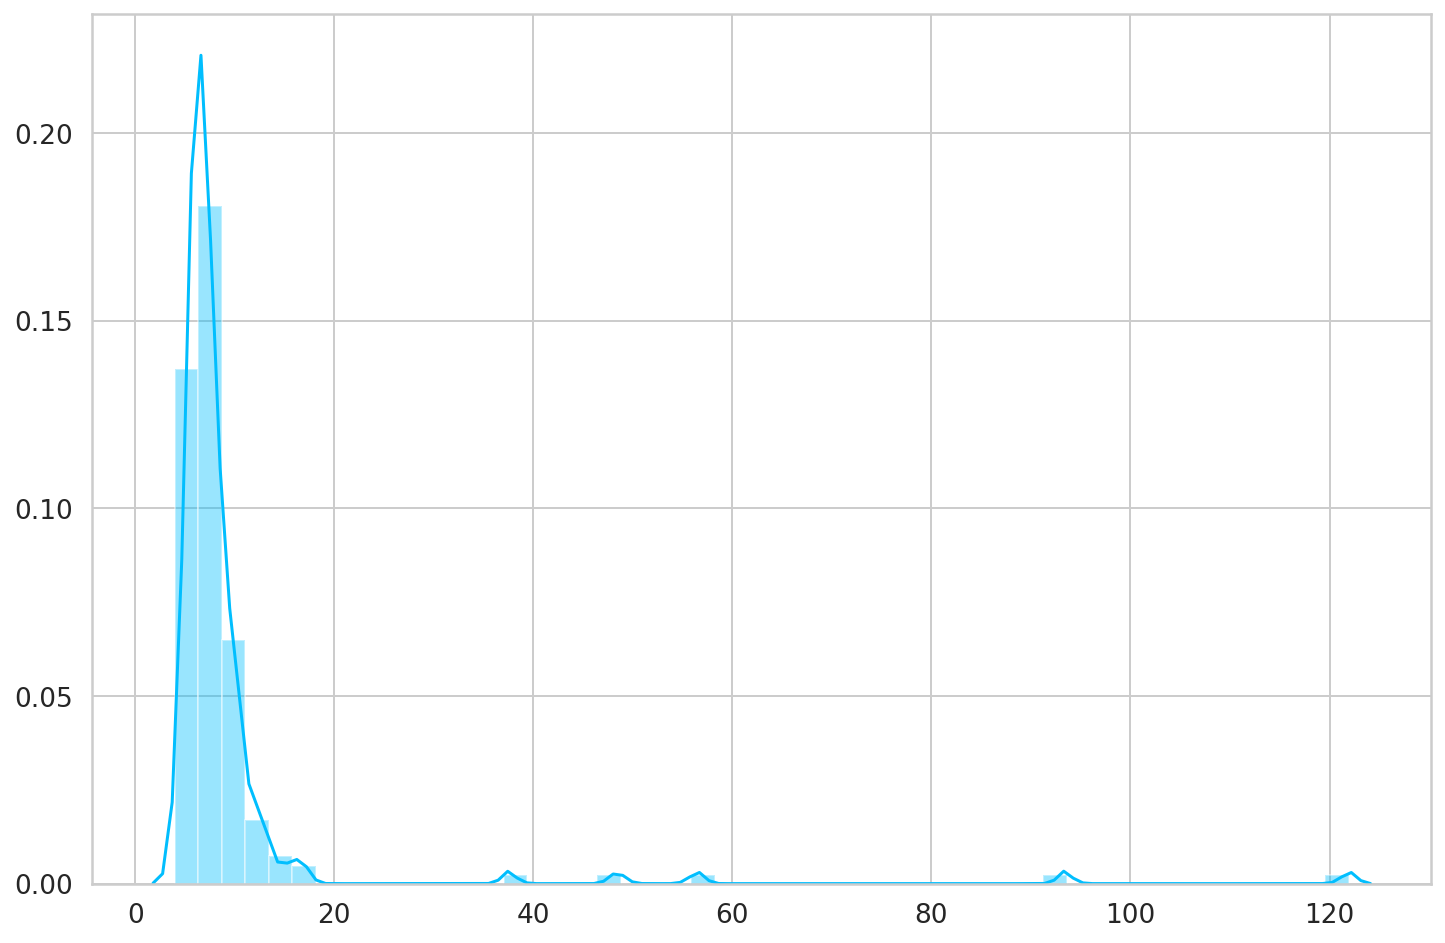
\includegraphics[width=0.7\textwidth]{images/attention_normal.png}
    \caption{LSTM Autoencoder with Attention: normal heartbeats loss distribution.}
\end{figure}
\begin{figure}[!t]
    \centering
    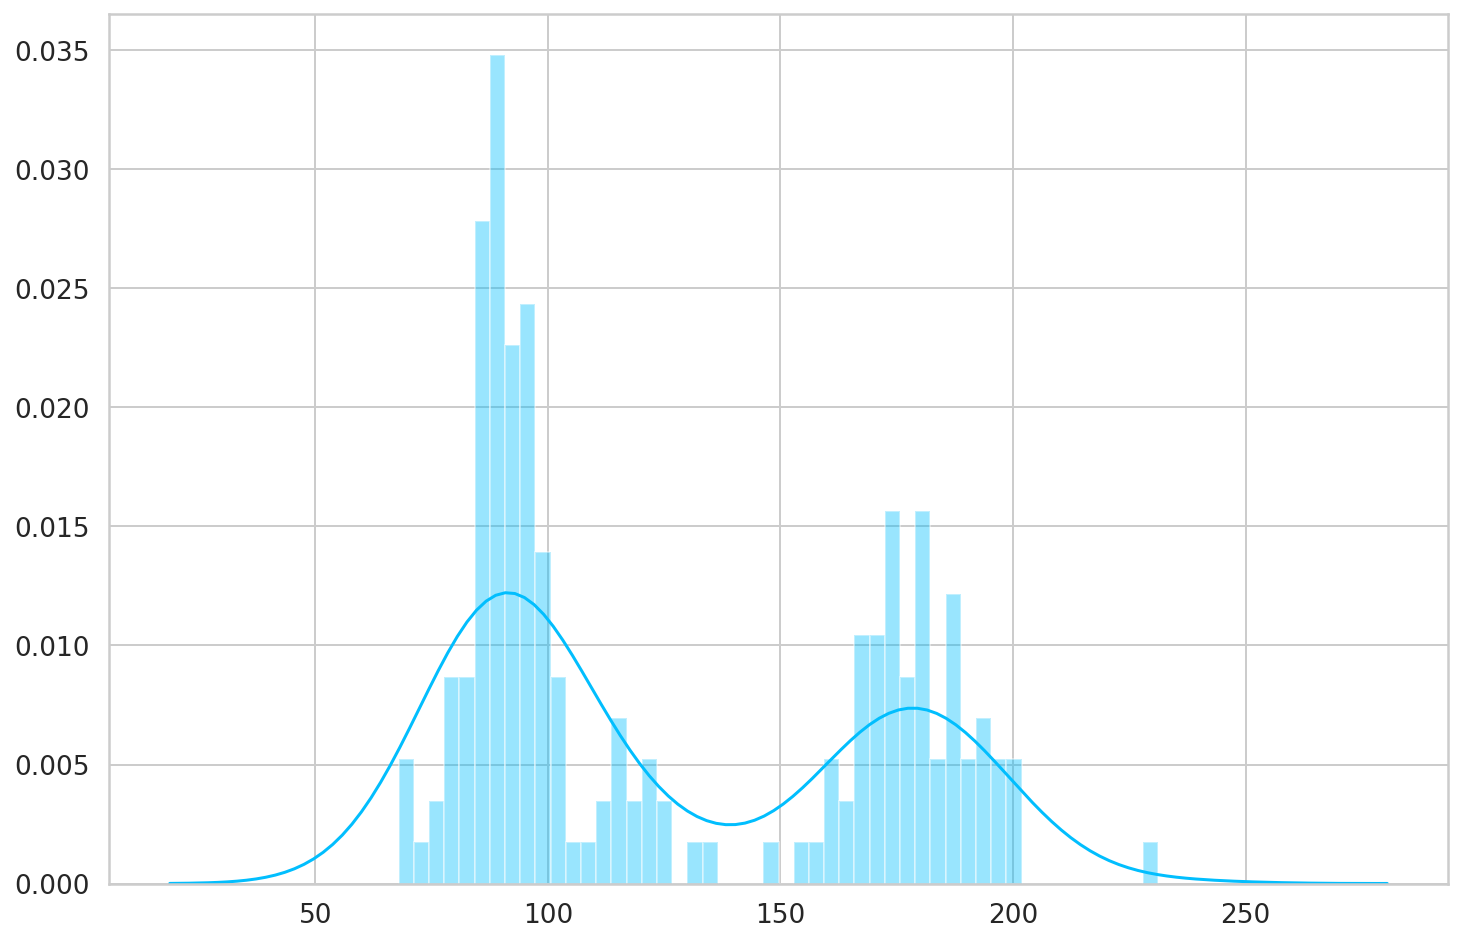
\includegraphics[width=0.7\textwidth]{images/attention_abnormal.png}
    \caption{LSTM Autoencoder with Attention: abnormal heartbeats loss distribution.}
\end{figure}
\begin{figure}[!t]
    \centering
    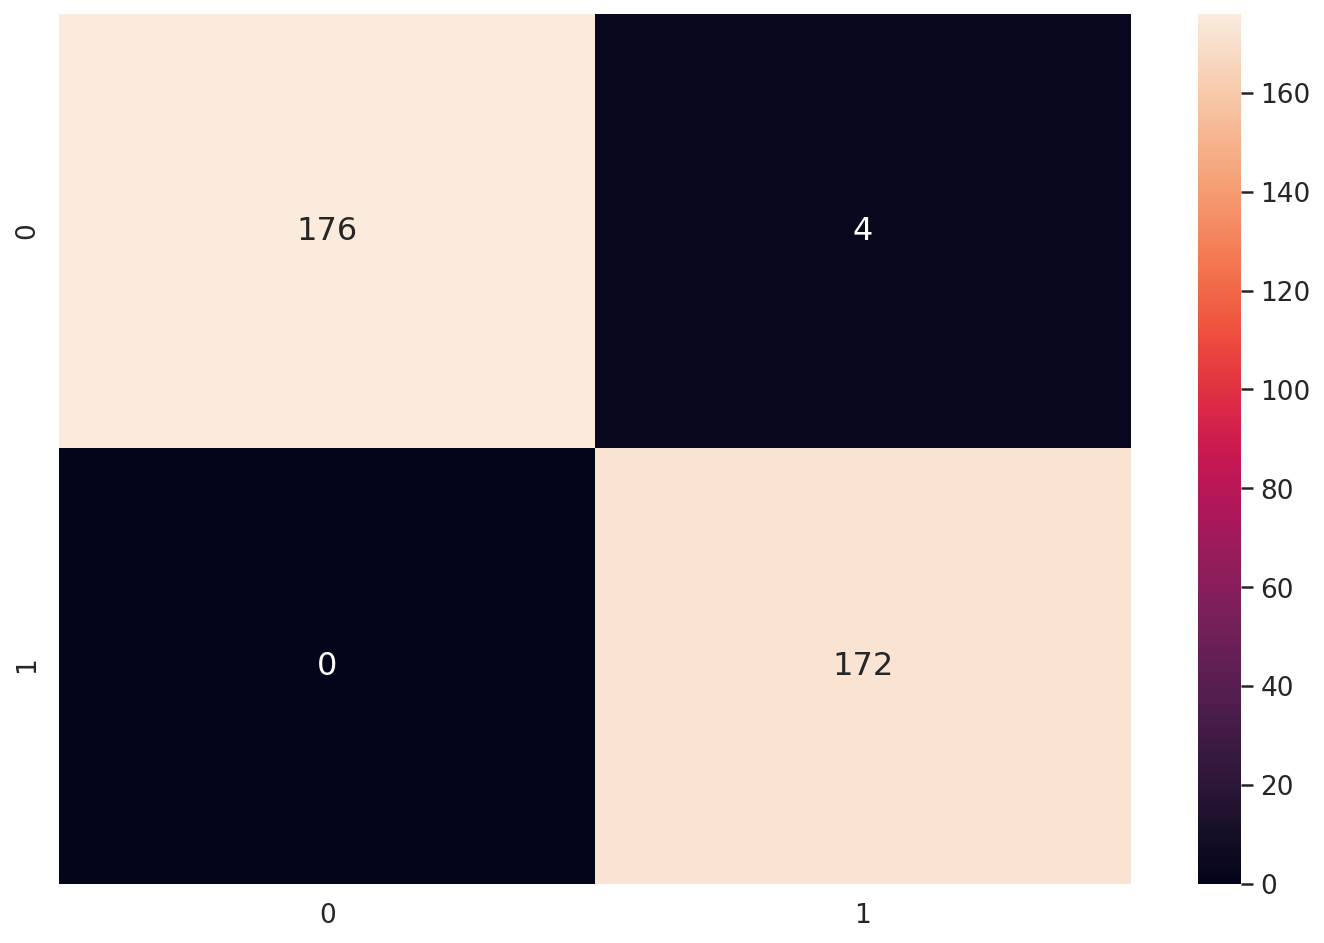
\includegraphics[width=0.7\textwidth]{images/attention_Cofmat.png}
    \caption{LSTM Autoencoder with Attention: Confusion Matrix.}
\end{figure}

\subsection{Transformer Model}
Transformer model behaves worse than LSTM autoencoders. In fact, Transformer model can't clearly distinguish normal heartbeats(loss distribution see Fig16) and abnormal heartbeats(loss distribution see Fig17), comparing with LSTM autoencoder, which allows a more narrow threshold range. The confusion matrix(Fig18) also tells us that transformer's error rate is higher. Besides, What the decoder reconstruct(Fig19) is similar to its original input data, meaning Transformer encoder isn't good at capturing features from the training normal data. For this case, transformer has a too powerful generalization ability to keep the normal data series as well as detecting abnormal ones.
\begin{figure}[!t]
    \centering
    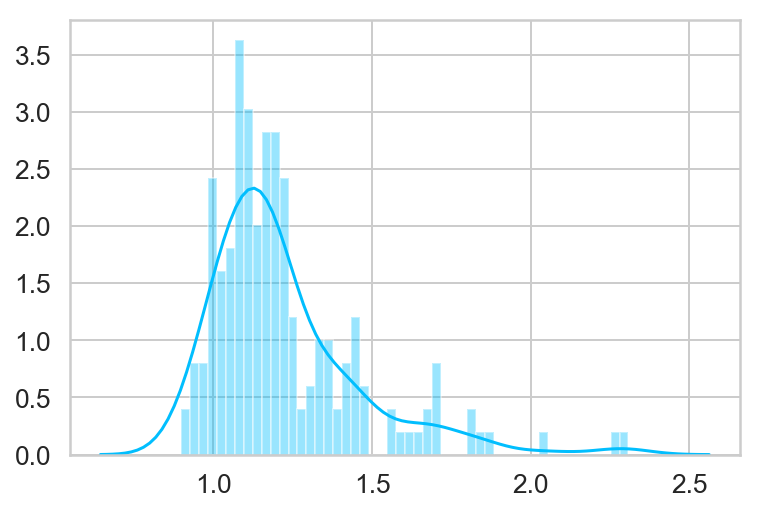
\includegraphics[width=0.7\textwidth]{images/transformer_normal.png}
    \caption{Transformer: Normal heartbeats loss distribution.}
\end{figure}
\begin{figure}[!t]
    \centering
    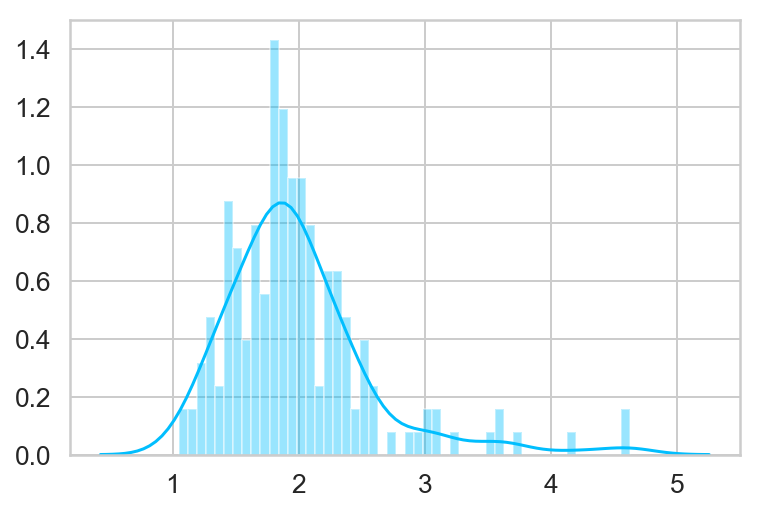
\includegraphics[width=0.7\textwidth]{images/transformer_abnormal.png}
    \caption{Transformer: Abnormal heartbeats loss distribution.}
\end{figure}
\begin{figure}[!t]
    \centering
    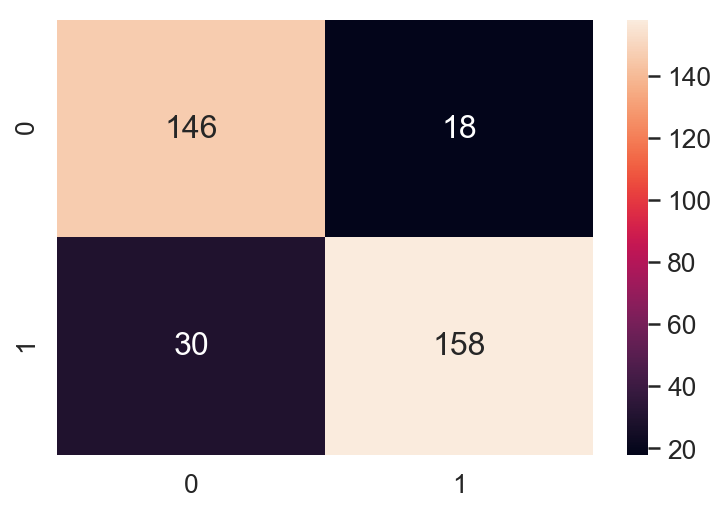
\includegraphics[width=0.7\textwidth]{images/transformer_Confmat.png}
    \caption{Transformer: Confusion Matrix.}
\end{figure}
\begin{figure}[!t]
    \centering
    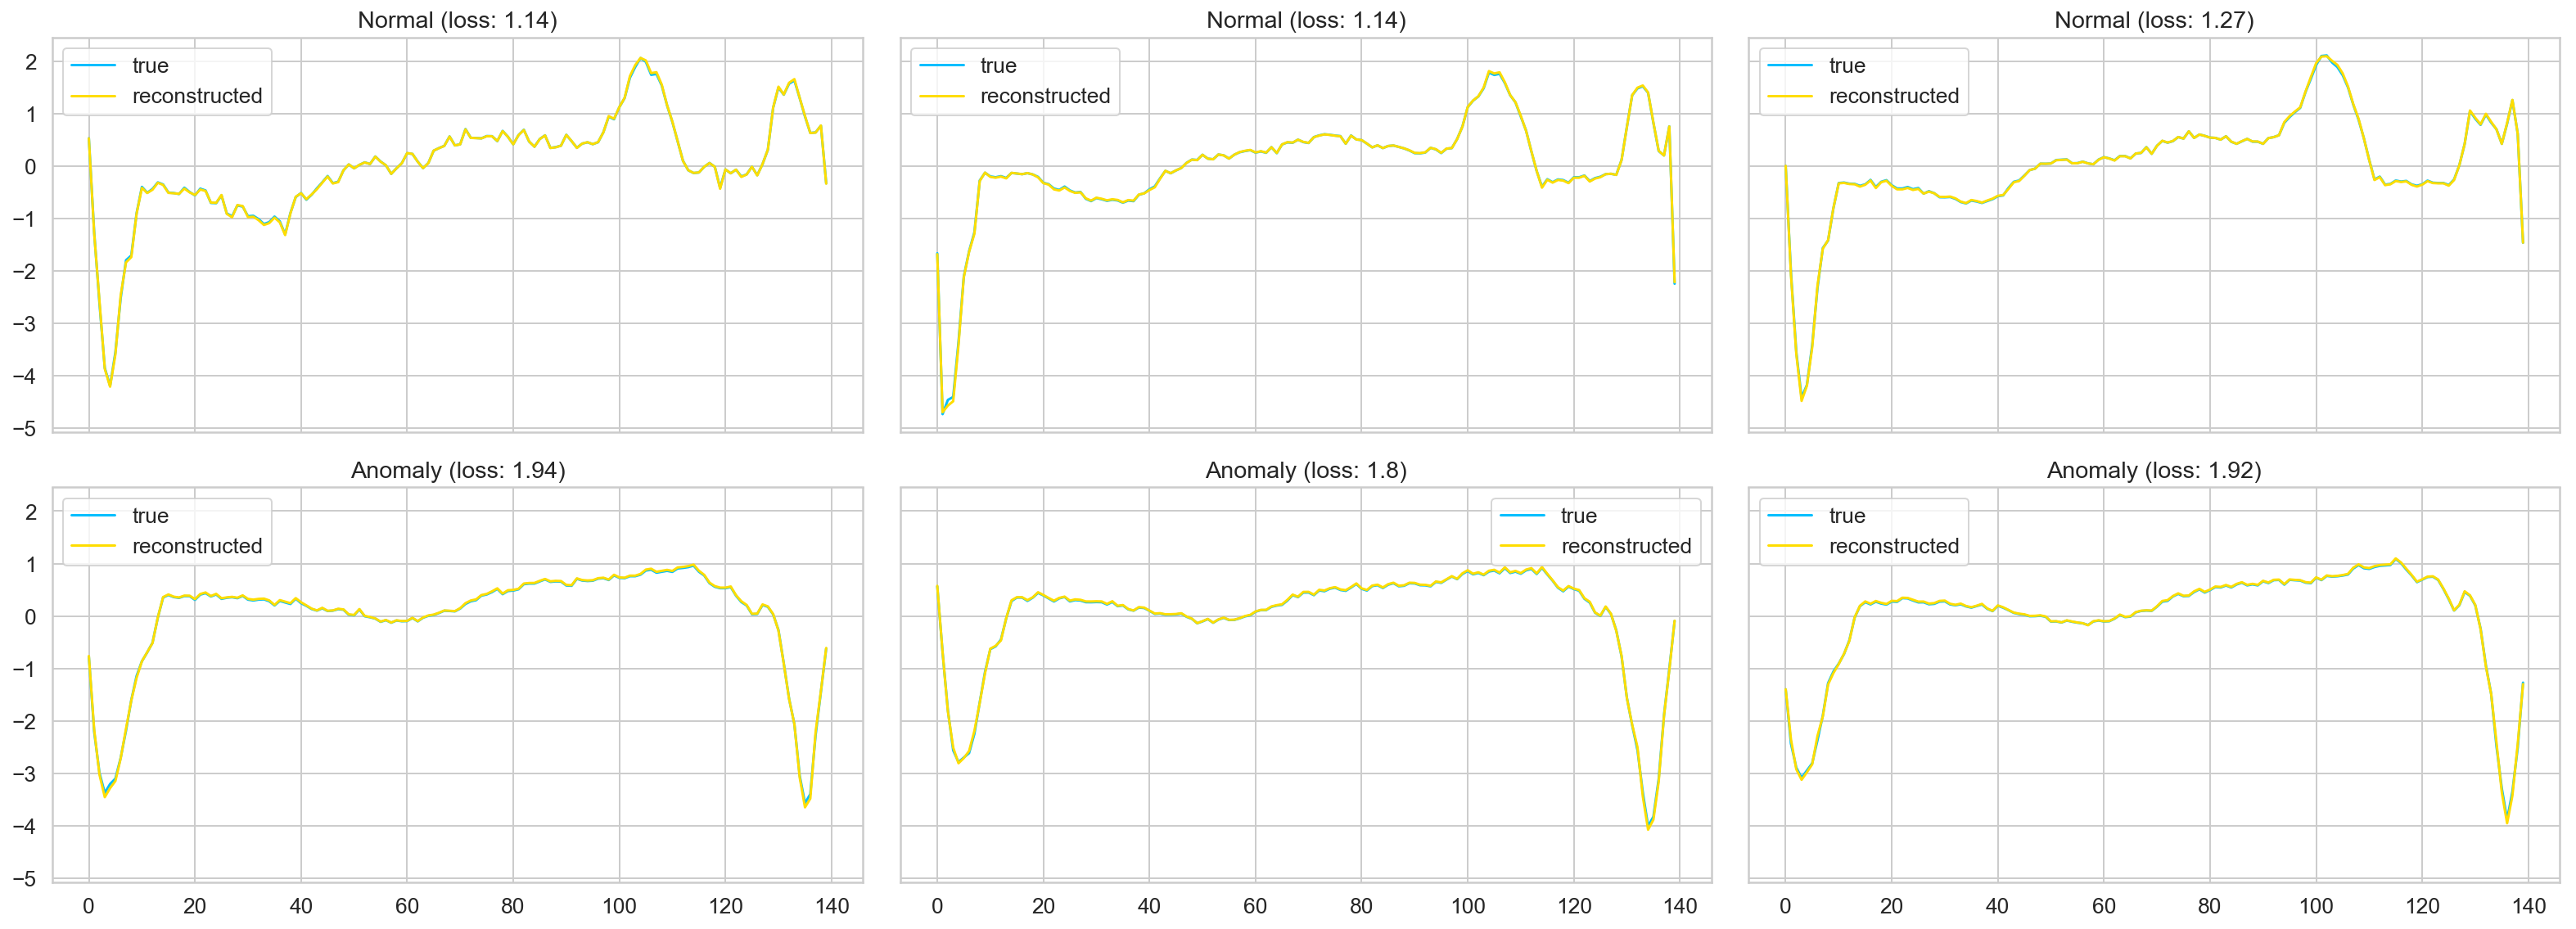
\includegraphics[width=1.0\textwidth]{images/transformer_reconstruct.png}
    \caption{Transformer: Test Data Decoder Reconstruction.}
\end{figure}

\section{Conclusion and Future Work}

\subsection{Conclusion}
Our work aims to develop a powerful model that can detect anomaly time series. We used the Electrocardiography data as a case study, and developed an LSTM variational recurrent autoencoder as a baseline to distinguish normal and abnormal time series with a 4 percent error rate. We further improved the model via attention mechanism, and obtain a better result for around 1 percent error rate. Furthermore, a Transformer model is also implemented, which could converge faster and smoother, but proves to be unsatisfactory in capturing normal data patterns as well as abnormal detection(13 percent error rate) comparing with LSTM autoencoder models, due to its non-symmetric nature and high generalization ability. 


\subsection{Future Work}
\begin{itemize}
    \item Collect, arrange, and interpolate more heart beat time series on the original website, and test the implemented models on a larger data sample, then use the trained model to serve as a useful tool in the historical time series data detection industry.
    
    \item Find more available data that has non-fixed length time series and lower dimensionality, and test if Transformer model could have a better behaviour than this case. 
\end{itemize}





%%%%%%%%%%%%%%%%%%%%%% Work Division %%%%%%%%%%%%%%%%%%%%%%
\section{Work Division}
The division of the work is showed below. For most of the work in this project, we will work together as a team.
The work division of the mid-term:
\begin{itemize}
    \item Dataset implementation: Ke Xu and Zhufeng Fan
    \item LSTM baseline and Transformer model implementation: Nicky Nocerino
    \item MLP baseline and Attention-based LSTM model implementation: Ke Xu
    \item Proposal and midterm report: Yilin Wang, Ke Xu, Zhufeng Fan, and Nicky Nocerino
    \item Code organization and maintenance: Ke Xu, Yilin Wang, Nicky Nocerino, and Zhufeng Fan
    \item Video presentation: Yilin Wang and Zhufeng Fan
    \item Final report: Zhufeng Fan and Yilin Wang
\end{itemize}


{
\bibliographystyle{unsrt}
\bibliography{egbib}
}

\end{document}
